\subsubsection{Test Service}\label{Testing:About:Service}
    In this section we will shortly describe the test service used for testing, \ref{attachment?}"EchoServiceLargeReply.war".
    % TODO: fix ref.

    The test service is very simple and deployable with GlassFish. It expects a request like this:
    \begin{figure}[h]
        \centering
        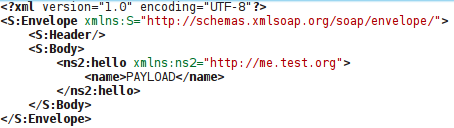
\includegraphics[width=\textwidth]{TestServiceRequest}
        \label{fig:TestServiceRequest}
    \end{figure}
    \\
    And responds like this:
    \begin{figure}[h]
        \centering
        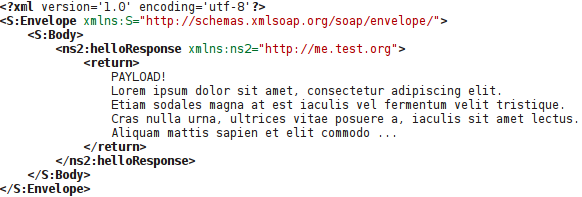
\includegraphics[width=\textwidth]{TestServiceResponse}
        \label{fig:TestServiceResponse}
    \end{figure}
    \\
    With PAYLOAD intact, and 10Kb of Lorem Ipsum\footnote{\url{http://www.lipsum.com/} - simply dummy text}. We add these 10Kb's of text to ensure that the response is considerably larger than the request, which should get us more realistic results when testing. We also sends the original payload back so the test client can easily identify which request was responded to. Those 10Kb of text also has a large impact on testing, it means that on lower than 10KBps bandwidth all the messages can't be sent in time. We chose to have it this way because it would give us a predictable test and also some static configuration on the ESB could be configured with this in mind.
